%TODO This is really ugly
The experiment is executed by directing a laser beam at a beam-splitter that splits the laser beam into two beams that takes different paths. The first path is held fixed and the second path may vary depending on how much a heated metal rod expands. The heated metal rod is held fixed at one end so that the metal rod only expand in one direction. This means that the varying path length decreases by two times the length the metal rod expands. The two beams then joins together and creates an interference pattern according to eq. \eqref{eq7}. The beams goes through some optics---that is only used to separate the interference fringes so that the photo diode can detect it---and then hits the photo diode, that measures the intensity.
A block diagram of the setup can be seen in fig. \ref{fig:blockSetup}.

\begin{figure}[htbp]
	\centering
	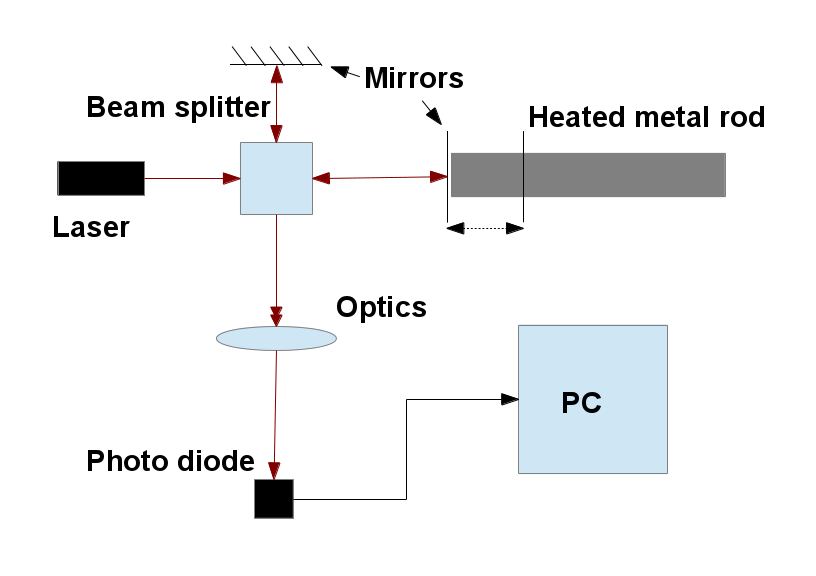
\includegraphics[width=0.8\textwidth]{img/blockSetup}
	\caption{Block diagram of the experimental setup.}
	\label{fig:blockSetup}
\end{figure}

\FloatBarrier
To determine the thermal expansion coefficient; we need to know the temperature of the rod, according to eq. \eqref{eq4}. Three thermistors measure the temperature and are fitted on the surface of the metal rod; one in the middle and one in each end of the rod. From this the temperature distribution of the metal rod can be approximated.